
%-----------------------------------------------------------------------------------------------------------------------------------------------%
%	The MIT License (MIT)
%
%	Copyright (c) 2021 Philip Empl
%
%	Permission is hereby granted, free of charge, to any person obtaining a copy
%	of this software and associated documentation files (the "Software"), to deal
%	in the Software without restriction, including without limitation the rights
%	to use, copy, modify, merge, publish, distribute, sublicense, and/or sell
%	copies of the Software, and to permit persons to whom the Software is
%	furnished to do so, subject to the following conditions:
%	
%	THE SOFTWARE IS PROVIDED "AS IS", WITHOUT WARRANTY OF ANY KIND, EXPRESS OR
%	IMPLIED, INCLUDING BUT NOT LIMITED TO THE WARRANTIES OF MERCHANTABILITY,
%	FITNESS FOR A PARTICULAR PURPOSE AND NONINFRINGEMENT. IN NO EVENT SHALL THE
%	AUTHORS OR COPYRIGHT HOLDERS BE LIABLE FOR ANY CLAIM, DAMAGES OR OTHER
%	LIABILITY, WHETHER IN AN ACTION OF CONTRACT, TORT OR OTHERWISE, ARISING FROM,
%	OUT OF OR IN CONNECTION WITH THE SOFTWARE OR THE USE OR OTHER DEALINGS IN
%	THE SOFTWARE.
%	
%
%-----------------------------------------------------------------------------------------------------------------------------------------------%


%============================================================================%
%
%	DOCUMENT DEFINITION
%
%============================================================================%

\documentclass[10pt,A4,english]{article}	


%----------------------------------------------------------------------------------------
%	ENCODING
%----------------------------------------------------------------------------------------

% we use utf8 since we want to build from any machine
\usepackage[utf8]{inputenc}		
\usepackage[USenglish]{isodate}
\usepackage{fancyhdr}
\usepackage[numbers]{natbib}
\usepackage[hidelinks]{hyperref}


%----------------------------------------------------------------------------------------
%	LOGIC
%----------------------------------------------------------------------------------------

% provides \isempty test
\usepackage{xstring, xifthen}
\usepackage{enumitem}
\usepackage[english]{babel}
\usepackage{blindtext}
\usepackage{pdfpages}
\usepackage{changepage}
%----------------------------------------------------------------------------------------
%	FONT BASICS
%----------------------------------------------------------------------------------------

% some tex-live fonts - choose your own

%\usepackage[defaultsans]{droidsans}
%\usepackage[default]{comfortaa}
%\usepackage{cmbright}
\usepackage[default]{raleway}
%\usepackage{fetamont}
%\usepackage[default]{gillius}
%\usepackage[light,math]{iwona}
%\usepackage[thin]{roboto} 

% set font default
\renewcommand*\familydefault{\sfdefault} 	
\usepackage[T1]{fontenc}

% more font size definitions
\usepackage{moresize}

%----------------------------------------------------------------------------------------
%	FONT AWESOME ICONS
%---------------------------------------------------------------------------------------- 

% include the fontawesome icon set
\usepackage{fontawesome}

% use to vertically center content
% credits to: http://tex.stackexchange.com/questions/7219/how-to-vertically-center-two-images-next-to-each-other
\newcommand{\vcenteredinclude}[1]{\begingroup
\setbox0=\hbox{\includegraphics{#1}}%
\parbox{\wd0}{\box0}\endgroup}
\newcommand{\tab}[1]{\hspace{.2\textwidth}\rlap{#1}}
% use to vertically center content
% credits to: http://tex.stackexchange.com/questions/7219/how-to-vertically-center-two-images-next-to-each-other
\newcommand*{\vcenteredhbox}[1]{\begingroup
\setbox0=\hbox{#1}\parbox{\wd0}{\box0}\endgroup}

% icon shortcut
\newcommand{\icon}[3] { 							
	\makebox(#2, #2){\textcolor{maincol}{\csname fa#1\endcsname}}
}	


% icon with text shortcut
\newcommand{\icontext}[4]{ 						
	\vcenteredhbox{\icon{#1}{#2}{#3}}  \hspace{2pt}  \parbox{0.9\mpwidth}{\textcolor{#4}{#3}}
}

% icon with website url
\newcommand{\iconhref}[5]{ 						
    \vcenteredhbox{\icon{#1}{#2}{#5}}  \hspace{2pt} \href{#4}{\textcolor{#5}{#3}}
}

% icon with email link
\newcommand{\iconemail}[5]{ 						
    \vcenteredhbox{\icon{#1}{#2}{#5}}  \hspace{2pt} \href{mailto:#4}{\textcolor{#5}{#3}}
}

%----------------------------------------------------------------------------------------
%	PAGE LAYOUT  DEFINITIONS
%----------------------------------------------------------------------------------------

% page outer frames (debug-only)
% \usepackage{showframe}		

% we use paracol to display breakable two columns
\usepackage{paracol}
\usepackage{tikzpagenodes}
\usetikzlibrary{calc}
\usepackage{lmodern}
\usepackage{multicol}
\usepackage{lipsum}
\usepackage{atbegshi}
% define page styles using geometry
\usepackage[a4paper]{geometry}

% remove all possible margins
\geometry{top=1cm, bottom=1cm, left=1cm, right=1cm}

\usepackage{fancyhdr}
\pagestyle{empty}

% space between header and content
% \setlength{\headheight}{0pt}

% indentation is zero
\setlength{\parindent}{0mm}

%----------------------------------------------------------------------------------------
%	TABLE /ARRAY DEFINITIONS
%---------------------------------------------------------------------------------------- 

% extended aligning of tabular cells
\usepackage{array}

% custom column right-align with fixed width
% use like p{size} but via x{size}
\newcolumntype{x}[1]{%
>{\raggedleft\hspace{0pt}}p{#1}}%


%----------------------------------------------------------------------------------------
%	GRAPHICS DEFINITIONS
%---------------------------------------------------------------------------------------- 

%for header image
\usepackage{graphicx}

% use this for floating figures
% \usepackage{wrapfig}
% \usepackage{float}
% \floatstyle{boxed} 
% \restylefloat{figure}

%for drawing graphics		
\usepackage{tikz}			
\usepackage{ragged2e}	
\usetikzlibrary{shapes, backgrounds,mindmap, trees}

%----------------------------------------------------------------------------------------
%	Color DEFINITIONS
%---------------------------------------------------------------------------------------- 
\usepackage{transparent}
\usepackage{color}

% primary color
\definecolor{maincol}{RGB}{ 64,64,64}

% accent color, secondary
% \definecolor{accentcol}{RGB}{ 250, 150, 10 }

% dark color
\definecolor{darkcol}{RGB}{ 70, 70, 70 }

% light color
\definecolor{lightcol}{RGB}{245,245,245}

\definecolor{accentcol}{RGB}{59,77,97}



% Package for links, must be the last package used
\usepackage[hidelinks]{hyperref}

% returns minipage width minus two times \fboxsep
% to keep padding included in width calculations
% can also be used for other boxes / environments
\newcommand{\mpwidth}{\linewidth-\fboxsep-\fboxsep}
	


%============================================================================%
%
%	CV COMMANDS
%
%============================================================================%

%----------------------------------------------------------------------------------------
%	 CV LIST
%----------------------------------------------------------------------------------------

% renders a standard latex list but abstracts away the environment definition (begin/end)
\newcommand{\cvlist}[1] {
	\begin{itemize}{#1}\end{itemize}
}

%----------------------------------------------------------------------------------------
%	 CV TEXT
%----------------------------------------------------------------------------------------

% base class to wrap any text based stuff here. Renders like a paragraph.
% Allows complex commands to be passed, too.
% param 1: *any
\newcommand{\cvtext}[1] {
	\begin{tabular*}{1\mpwidth}{p{1.05\mpwidth}}
		\parbox{1\mpwidth}{#1}
	\end{tabular*}
}
\newcommand{\cvtextsmall}[1] {
	\begin{tabular*}{0.8\mpwidth}{p{0.8\mpwidth}}
		\parbox{0.8\mpwidth}{#1}
	\end{tabular*}
}
%----------------------------------------------------------------------------------------
%	CV SECTION
%----------------------------------------------------------------------------------------

% Renders a a CV section headline with a nice underline in main color.
% param 1: section title
\newcommand{\cvsection}[1] {
	\vspace{14pt}
	\cvtext{
		\textbf{\LARGE{\textcolor{darkcol}{#1}}}\\[-4pt]
		\textcolor{accentcol}{ \rule{0.2\textwidth}{1.5pt} } \\
	}
}

\newcommand{\cvsectionsmall}[1] {
	\vspace{14pt}
	\cvtext{
		\textbf{\Large{\textcolor{darkcol}{#1}}}\\[-4pt]
		\textcolor{accentcol}{ \rule{0.2\textwidth}{1.5pt} } \\
	}
}

\newcommand{\cvheadline}[1] {
	\vspace{16pt}
	\cvtext{
		\textbf{\Huge{\textcolor{accentcol}{#1}}}\\[-4pt]
		 
	}
}

\newcommand{\cvsubheadline}[1] {
	\vspace{16pt}
	\cvtext{
		\textbf{\huge{\textcolor{darkcol}{#1}}}\\[-4pt]
		 
	}
}
%----------------------------------------------------------------------------------------
%	META SKILL
%----------------------------------------------------------------------------------------

% Renders a progress-bar to indicate a certain skill in percent.
% param 1: name of the skill / tech / etc.
% param 2: level (for example in years)
% param 3: percent, values range from 0 to 1
\newcommand{\cvskill}[3] {
	\begin{tabular*}{1\mpwidth}{p{0.72\mpwidth}  r}
 		\textcolor{black}{\textbf{#1}} & \textcolor{maincol}{#2}\\
	\end{tabular*}%
	
	\hspace{4pt}
	\begin{tikzpicture}[scale=1,rounded corners=2pt,very thin]
		\fill [lightcol] (0,0) rectangle (1\mpwidth, 0.15);
		\fill [accentcol] (0,0) rectangle (#3\mpwidth, 0.15);
  	\end{tikzpicture}%
}


%----------------------------------------------------------------------------------------
%	 CV EVENT
%----------------------------------------------------------------------------------------

% Renders a table and a paragraph (cvtext) wrapped in a parbox (to ensure minimum content
% is glued together when a pagebreak appears).
% Additional Information can be passed in text or list form (or other environments).
% the work you did
% param 1: time-frame i.e. Sep 14 - Jan 15 etc.
% param 2:	 event name (job position etc.)
% param 3: Customer, Employer, Industry
% param 4: Short description
% param 5: work done (optional)
% param 6: technologies include (optional)
% param 7: achievements (optional)
\newcommand{\cvevent}[7] {
	
	% we wrap this part in a parbox, so title and description are not separated on a pagebreak
	% if you need more control on page breaks, remove the parbox
	\parbox{\mpwidth}{
		\begin{tabular*}{1\mpwidth}{p{0.71\mpwidth}  r}
	 		\textcolor{black}{\textbf{#2}} & \colorbox{accentcol}{\makebox[0.3\mpwidth]{\textcolor{white}{\textbf{#1}}}} \\
			\textcolor{maincol}{#3} & \\
		\end{tabular*}\\[8pt]
	
		\ifthenelse{\isempty{#4}}{}{
			\cvtext{#4}\\
		}
	}
	\vspace{14pt}
}


%----------------------------------------------------------------------------------------
%	 CV META EVENT
%----------------------------------------------------------------------------------------

% Renders a CV event on the sidebar
% param 1: title
% param 2: subtitle (optional)
% param 3: customer, employer, etc,. (optional)
% param 4: info text (optional)
\newcommand{\cvmetaevent}[4] {
	\textcolor{maincol} { \cvtext{\textbf{\begin{flushleft}#1\end{flushleft}}}}

	\ifthenelse{\isempty{#2}}{}{
	\textcolor{black} {\cvtext{\textbf{#2}} }
	}

	\ifthenelse{\isempty{#3}}{}{
		\cvtext{{ \textcolor{maincol} {#3} }}\\
	}

	\cvtext{#4}\\[14pt]
}

%---------------------------------------------------------------------------------------
%	QR CODE
%----------------------------------------------------------------------------------------

% Renders a qrcode image (centered, relative to the parentwidth)
% param 1: percent width, from 0 to 1
\newcommand{\cvqrcode}[1] {
	\begin{center}
		\includegraphics[width={#1}\mpwidth]{qrcode}
	\end{center}
}


% HEADER AND FOOOTER 
%====================================
\newcommand\Header[1]{%
\begin{tikzpicture}[remember picture,overlay]
\fill[accentcol]
  (current page.north west) -- (current page.north east) --
  ([yshift=50pt]current page.north east|-current page text area.north east) --
  ([yshift=50pt,xshift=-3cm]current page.north|-current page text area.north) --
  ([yshift=10pt,xshift=-5cm]current page.north|-current page text area.north) --
  ([yshift=10pt]current page.north west|-current page text area.north west) -- cycle;
\node[font=\sffamily\bfseries\color{white},anchor=west,
  xshift=0.7cm,yshift=-0.32cm] at (current page.north west)
  {\fontsize{12}{12}\selectfont {#1}};
\end{tikzpicture}%
}

\newcommand\Footer[1]{%
\begin{tikzpicture}[remember picture,overlay]
\fill[lightcol]
  (current page.south east) -- (current page.south west) --
  ([yshift=-80pt]current page.south east|-current page text area.south east) --
  ([yshift=-80pt,xshift=-6cm]current page.south|-current page text area.south) --
  ([xshift=-2.5cm,yshift=-10pt]current page.south|-current page text area.south) --	
  ([yshift=-10pt]current page.south east|-current page text area.south east) -- cycle;
\node[yshift=0.32cm,xshift=9cm] at (current page.south) {\fontsize{10}{10}\selectfont \textbf{\thepage}};
\end{tikzpicture}%
}


%=====================================
%============================================================================%
%
%
%
%	DOCUMENT CONTENT
%
%
%
%============================================================================%
\begin{document}

\columnratio{0.31}
\setlength{\columnsep}{2.2em}
\setlength{\columnseprule}{4pt}
\colseprulecolor{white}


% LEBENSLAUF HIERE
\AtBeginShipoutFirst{\Header{CV}\Footer{1}}
\AtBeginShipout{\AtBeginShipoutAddToBox{\Header{CV}\Footer{2}}}

\newpage

\colseprulecolor{lightcol}
\columnratio{0.31}
\setlength{\columnsep}{2.2em}
\setlength{\columnseprule}{4pt}
\begin{paracol}{2}


\begin{leftcolumn}
%---------------------------------------------------------------------------------------
%	META IMAGE
%----------------------------------------------------------------------------------------
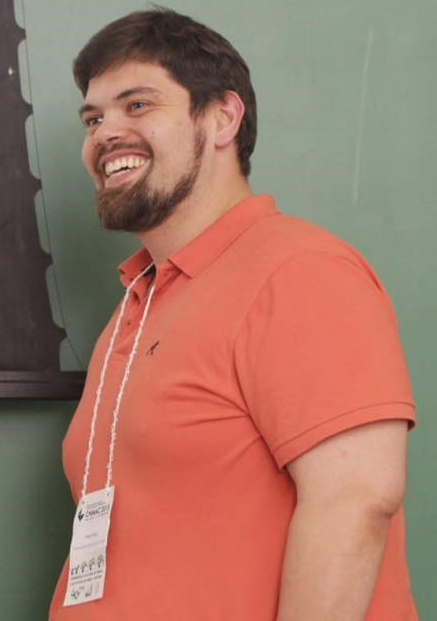
\includegraphics[width=\linewidth]{resources/fidalgo.png}	%trimming relative to image size

%---------------------------------------------------------------------------------------
%	META SKILLS
%----------------------------------------------------------------------------------------
	\fcolorbox{white}{white}{\begin{minipage}[c][4.5cm][c]{1\mpwidth}
		\LARGE{\textbf{\textcolor{maincol}{Felipe Fidalgo}}} \\[2pt]
		\normalsize{ \textcolor{maincol} {Assistant Professor} }
		%
		\\[6pt]
		%
		\small{ \textcolor{black} {Universidade Federal de Santa Catarina} }
		%
		\\[6pt]
		%
		\small{ \textcolor{black} {School of Technology, Exact Sciences and Education} }
		%
		\\[6pt]
		%
		\small{ \textcolor{black} {Department of Mathematics} }
		%
		\\[6pt]
		%
		\small{ \textcolor{black} {Blumenau -- Santa Catarina -- Brazil} }
\end{minipage}} \\

\cvsection{Contact}

\icontext{MapMarker}{16}{880 Marechal Rondon street \\ Room B204 \\ zip code 89065 -- 200 \\ Blumenau, Brazil}{black}
\\[6pt]
\icontext{Phone}{16}{+55 047 3080 0471}{black}
\\[6pt]
\iconemail{Envelope}{16}{felipe.fidalgo@ufsc.br}{XXXX@XXXXX.XX}{black}
\\[6pt]
\iconhref{Home}{16}{felipefidalgo.paginas.ufsc.br}{felipefidalgo.paginas.ufsc.br}{black}
\\

\cvsection{Research Interests}

\icontext{CaretRight}{12}{Distance Geometry and Its \\ Applications}{black}\\[6pt]
\icontext{CaretRight}{12}{Optimization}{black}\\[6pt]
\icontext{CaretRight}{12}{Semidefinite Programming}{black}\\[6pt]
\icontext{CaretRight}{12}{Quaternions and Applications}{black}\\[6pt]
\icontext{CaretRight}{12}{Clifford Algebras and Applications}{black}\\[6pt]
\icontext{CaretRight}{12}{Molecular Geometry}{black}\\[6pt]
\icontext{CaretRight}{12}{Bioinformatics}{black}\\[6pt]
\icontext{CaretRight}{12}{Discrete Mathematics}{black}\\[6pt]
\icontext{CaretRight}{12}{Operations Research}{black}\\[6pt]

% [6pt]
% \iconhref{Github}{16}{github.com/username}{https://www.github.com/username}{black}\\[6pt]
% \iconhref{Xing}{16}{xing.com/user\_name}{https://www.xing.com/profile/User_Name}{black}\\


% \icontext{CaretRight}{12}{Universidade Federal de Santa Catarina}{black}\\[6pt]
% \icontext{CaretRight}{12}{german}{black}\\[6pt]
% \icontext{CaretRight}{12}{unmarried}{black}\\[6pt]



% \cvsection{Skills}

% \cvskill{Software development} {6+ Jahre} {1} \\[-2pt]

% \cvskill{Cyber security} {4+ yrs.} {0.64} \\[-2pt]

% \cvskill{Internet business/ \newline E-commerce} {4+ yrs.} {0.64} \\[-2pt]

% \cvskill{Web development} {2+ yrs.} {0.32} \\[-2pt]

% \cvskill{Big data/ \newline Data science} {2+ yrs.} {0.32} \\[-2pt]

% \cvskill{Distributed legder \newline technology} {2+ yrs.} {0.32} \\[-2pt]

% \cvskill{Internet of things} {1+ yrs.} {0.16} \\[-2pt]

% \cvskill{Cloud computing} {1+ yrs.} {0.16} \\[-2pt] \\

% \cvskill{German} {L1} {1} \\[-2pt]

% \cvskill{English} {C1} {0.9} \\[-2pt]

\newpage
%---------------------------------------------------------------------------------------
%	EDUCATION
%----------------------------------------------------------------------------------------
\cvsection{Education}

\cvmetaevent
{03/2011 - 02/2015}
{Applied Mathematics (Ph.D)}
{University of Campinas (UNICAMP)}
{\textit{PhD's~thesis:} 
\\ 
%
``Dividing-and-conquering with symmetries in Distance Geometry'' 
\\[7pt] 
%
\textit{Supervisor:} Prof. Carlile Lavor, PhD
\\
\textit{Awarded on:} Feb.~27th, 2015
\\[7pt]
\textit{Examiners:} \\ Sueli Costa, Eduardo Miqueles, Giuliano Guardia and Tiberius Bonates.
\\[7pt] 
%
\textit{Distance Geometry • Clifford Algebra}}
%
\cvmetaevent
{03/2009 - 05/2011}
{Applied Mathematics (M.Sc)}
{University of Campinas (UNICAMP)}
{\textit{Master's thesis:} 
\\ 
%
``Algorithms for problems in Molecular Geometry'' 
\\[7pt] 
%
\textit{Supervisor:} Prof. Carlile Lavor, PhD
\\
\textit{Awarded on:} May~13rd, 2011
\\[7pt]
\textit{Examiners:} \\ Luiz Ochi and Márcia Ruggiero.
\\[7pt] 
%
\textit{Distance Geometry • Bioinformatics}}
%
\cvmetaevent
{03/2005 - 12/2008}
{Mathematics (B.Sc)}
{Universidade Paulista ``Julio de Mesquita Filho'' (UNESP)}
% {\textit{Field 1 • Field 2} \newline Bachelor's thesis: \glqq title of Master's thesis\grqq.}


%
%\cvsection{Projekte}

%	\cvlist{
%		\item \hyperlink{https://github.com/philipempl/ether-twin}{\textbf{Ether-Twin.}}\\ Ethereum Applikation für Digital Twins.
%		\item \hyperlink{https://github.com/philipempl/Peter-Pan}{\textbf{Peter Pan.}}\\ Koch-App (t.b.a.).
%		\item \hyperlink{https://github.com/philipempl/Innovation-Tool}{\textbf{Innovation Tool.}}\\ Webcrawler für \hyperlink{https://ibi.de/}{Ibi}.
%		\item \hyperlink{https://github.com/philipempl/cozone}{\textbf{COZONE.}} \\ Soziales Netzwerk (t.b.a.).
%		\item \hyperlink{https://github.com/geritwagner/enlit}{\textbf{ENLIT.}}\\ Exploring new Literature (Bachelorarbeit).
%		\item \textbf{Crowdfunding.} \\Modul mit \hyperlink{https://senacor.com/}{Senacor} für \hyperlink{https://www.paydirekt.de/}{paydirekt}.
%		}


% \cvsection{Interests}

% \icontext{CaretRight}{12}{Guitarist}{black}\\[6pt]
% \icontext{CaretRight}{12}{DIY}{black}\\[6pt]
% \icontext{CaretRight}{12}{Fitness}{black}\\[6pt]
% \icontext{CaretRight}{12}{Cooking}{black}\\[6pt]
% \icontext{CaretRight}{12}{Travel}{black}\\[6pt]


% \cvsection{Contact}

% \icontext{MapMarker}{16}{Street name XX\\D-XXXXX Lorem}{black}\\[6pt]
% \icontext{MobilePhone}{16}{+XX XXX XXXX XXXX}{black}\\[6pt]
% \iconemail{Envelope}{16}{XXXX@XXXXX.XX}{XXXX@XXXXX.XX}{black}\\[6pt]
% \iconhref{Home}{16}{XXX.XXX-XXXX.XX}{http://XXX-XXX.XXX.XX}{black}\\[6pt]
% \iconhref{Github}{16}{github.com/username}{https://www.github.com/username}{black}\\[6pt]
% \iconhref{Xing}{16}{xing.com/user\_name}{https://www.xing.com/profile/User_Name}{black}\\

	
%\cvqrcode{0.3}

\end{leftcolumn}
\begin{rightcolumn}
%---------------------------------------------------------------------------------------
%	TITLE  HEADER
%----------------------------------------------------------------------------------------


%---------------------------------------------------------------------------------------
%	PROFILE
%----------------------------------------------------------------------------------------
\cvsection{Biography}
\vspace{4pt}

\cvtext{
Felipe Fidalgo was born in Andradina, state of Sao Paulo, Brazil, on February, 1st, 1987. 
%
He is a Bachelor of Mathematics (2008) and M.Sc.~(2011)~and~Ph.D.~(2015)~in Applied Mathematics 
at University of Campinas, whose main research themes were Distance Geometry with applications 
in Molecular Geometry and Clifford Algebras. 
%
Since 2015, he is professor of the Department of Mathematics at Blumenau Campus of the 
Universidade Federal de Santa Catarina, leading research projects, teaching and supervising projects 
both in undergraduate and in graduate levels and developing relevant administration tasks.
%
Currently, he is visiting scholar at University of Waterloo, Canada. 
}


\bigskip 

%---------------------------------------------------------------------------------------
%	WORK EXPERIENCE
%----------------------------------------------------------------------------------------

\vspace{10pt}
\cvsection{Work experience}
\vspace{4pt}


\cvevent
{Oct/2015 - today}
	{Assistant Professor}
	{Department of Mathematics\newline School of Technology, Exact Sciences and Education (CTE)\newline Campus of Blumenau, Blumenau, Brazil\newline Universidade Federal de Santa Catarina (UFSC)}
	{Fidalgo lectures mathematical courses for Mathematics, Chemistry and Engineering undergraduate programs which are held in the campus. 
	%
	Also, he works as a lecturer, supervisor, co-coordinator (two terms) and coordinator (two terms) in PROFMAT (Graduate), which is an professional Master's in Mathematics. 
	%
	And, he develops research projects which involve colleagues and undergraduate and graduate students; supervisions are involved in this task.
	%
	His position is as Assistant Professor, the initial full-time one in the tenure track of the Federal system (public) of Universities in Brazil.}
	\vfill\null

\bigskip 

\cvevent
{Aug/2025 - today}
	{Research Scholar}
	{Department of Combinatorics and Optimization
	\newline 
	Faculty of Mathematics
	\newline 
	University of Waterloo}
	{Fidalgo is currently visiting Prof.~Henry Wolkowicz
	to perform research projects on Optimization and
	Semidefinite Programming.}
	\vfill\null

\bigskip 

\cvevent
{Aug/2015 - Sep/2015}
	{Instructor}
	{Department of Mathematics \\ School of Engineering of Ilha Solteira (FEIS)\newline Campus of Ilha Solteira, Ilha Solteira, Brazil \newline Universidade Estadual ``Julio de Mesquita Filho'' (UNESP)}
	{He was hired to lecture Calculus courses for the Engineering undergraduate programs in this campus as a part-time substitute instructor, a non-ternure-track position in a public institution.}
	\vfill\null

\bigskip 

\cvevent
{Feb/2014 - Oct/2015}
	{Instructor}
	{Faculdades Integradas ``Rui Barbosa''~(FIRB)\newline Andradina, Brazil}
	{He lectured Calculus, Linear Algebra, Differential Equations, Numerical Methods and Financial Mathematics for Engineering and Business undergraduate programs. It is a non-ternure-track position in a private institution. This was the first teaching experience of him in academic courses.}
	\vfill\null

\bigskip 

\cvsection{Prizes}

\begin{itemize}[leftmargin=*]

\item Nominee for Hestenes' Prize (2018) \medskip \\ Second position was awarded in the finale of the Hestenes Prize (top 3) during AGACSE 2018 in Campinas, Brazil.

\medskip 

\item Nominee for DGP "Top Five Papers" (2013) \medskip \\ Fourth position was awarded in the finale of the DGP "Top Five Papers" during Workshop on Distance Geometry and Applications (DGP) 2013 in Manaus, Brazil.

\end{itemize}

%\newpage 

\cvsection{Publications}

\begin{itemize}[leftmargin=*]

\item \textbf{Fidalgo,~F.} \& Philippi,~G. \& Castelani,~E.~V. 
\& Nack,~F.~A. (2025). \\ 
\href{https://drive.google.com/file/d/1XyeFNhor3UIy8hiweu895VoyY0SOQMnC/view}
{"A Long-Short-Term Memory neural network applied to a problem 
of classification using molecular-driven structures."}. 
In: \textit{Proceedings of the XIV Regional Applied and Computational 
Mathematics Meeting (XIV ERMAC Parana)}, pp.~137--139, Maringa, Brazil. 
(Expanded Abstract)
%
\\[5pt]
%
\item Haag, S. \& \textbf{Fidalgo, F.} (2024).
\href{ https://doi.org/10.35819/remat2025v11id7227 }{"Distance Geometry as an approach for High School within the context of the Brazilian National Common Core Curriculum".} 
\textit{Electronic Journal of Mathematics (REMAT)} 11, e201-1 -- e201-25.
%
\\[5pt]
%
\item \textbf{Fidalgo, F.} \& Castelani,~E.V. \& Philippi, G. (2023). \href{https://doi.org/10.1007/s10589-023-00526-8}{"A numerical-and-computational study on the impact of using Quaternions in the Branch-and-Prune Algorithm for exact discretizable distance geometry problems".} \textit{Computational Optimization and Applications} 87 (2), 501-530.
%
\\[5pt]
%
\item De Camargo,~V.S. \& Castelani,~E.V. \&  Fernandes,~L.A.F. \& \textbf{Fidalgo,~F.} (2019). \href{https://doi.org/10.1007/s00006-019-0995-7}{"Geometric Algebra to Describe the Exact Discretizable Molecular Distance Geometry Problem for an Arbitrary Dimension".} \textit{Advances in Applied Clifford Algebra (AACA)} 29(4), 75. 
%
\\[5pt]
%
\item \textbf{Fidalgo,~F.} (2018). \\ "Using quaternion geometric algebra for efficient rotations in the branch‐and‐prune algorithm   to solve the discretizable molecular distance geometry problem". In: \textit{Proceedings of the 7th Conference on Applied Geometric Algebra in Computer Science and Engineering (AGACSE)}, Campinas, Brazil, July 23-27.~(Nominee to the Hestenes Prize and awarded with the second position)
%
\\[5pt]
%
\item \textbf{Fidalgo,~F.} \& Gonçalves,~D.G. \& Lavor,~C. \& Liberti,~L. \& Mucherino,~A. (2018). \href{https://doi.org/10.1007/s10898-018-0610-9}{"A symmetry-based splitting strategy for discretizable distance geometry problems".} In: \textit{Journal of Global Optimization (JOGO)} 71, 717-733. (D.O.I.~10.1007/s10898-018-0610-9)
%
\\[5pt]
%
\item Rodriguez,~J.E.A. \& \textbf{Fidalgo,~F.} (2015). \\ "The problem of Square-Base Pyramid". In: \textit{C.Q.D. Electronic Paulista Journal} 4, 47-54.
%
\\[5pt]
%
\item \textbf{Fidalgo,~F.} \& Lavor,~C. (2015). \\ "Deciding Directions for the Branch-and-Prune Algorithm using gaps - a worst-case analysis". In: \textit{Proceedings of the Mathematical Methods and Modeling of Biophysical Phenomena Workshop (BIOMATH)}, Cabo Frio, Brazil, March 2-7. (Abstract)
%
\\[5pt]
%
\item \textbf{Fidalgo,~F.} \& Rodriguez,~J.E.A. (2014). \\ "A new approach to split Discretizable Molecular Distance Geometry Problem using gaps". In: \textit{Proceedings of XXXV National Conference on Applied and Computational Mathematics (CNMAC)}, Natal, Brazil, September 08-12.
%
\\[5pt]
%
\item Rodriguez,~J.E.A. \& \textbf{Fidalgo,~F.} (2014). \\ "The problem of Square-Base Pyramid". In: \textit{Proceedings of XXXV National Conference on Applied and Computational Mathematics (CNMAC)}, Natal, Brazil, September 08-12.
%
\\[5pt]
%
\item \textbf{Fidalgo,~F.} \& Rodriguez,~J.E.A. (2014). \\ "Exploiting Symmetries in a divide-and-conquer approach for solving the DMDGP". In: \textit{Proceedings of the Many Faces of Distances}, Campinas, Brazil. (Expanded Abstract)
%
\\[5pt]
%
\item \textbf{Fidalgo,~F.} \& Rodriguez,~J.E.A. (2013). \\ "Quaternions as a tool for merging multiple realization trees". In: \textit{Proceedings of the Workshop on Distance Geometry and Applications (DGA)}, Manaus, Brazil.
%
\\[5pt]
%
\item \textbf{Fidalgo,~F.} \& Maioli,~D. \& Abreu,~E. (2013). \\ " Updated T Algorithm for the resolution of Molecular Distance Geometry Problems by means of linear systems". In: \textit{Proceedings of the Workshop on Distance Geometry and Applications (DGA)}, Manaus, Brazil.
%
\\[5pt]
%
\item \textbf{Fidalgo,~F.} \& Maioli,~D. \& Abreu,~E. \& Lavor,~C. (2012). \\ "A numerical formulation for the resolution of Molecular Distance Geometry Problems". In: \textit{Proceedings of the joint Conference Congresso Latino-Iberoamericano de Investigacion Operativa/Simpósio Brasileiro de Pesquisa Operacional (CLAIO/SBPO)}, Rio de Janeiro, Brazil.
%
\\[5pt]
%
\item \textbf{Fidalgo,~F.} (2012). \\ "Algoritmos para a Resolução de Problemas de Geometria Molecular". In: \textit{Proceedings of XVI Escuela Latinoamericana de Verano en Investigación Operativa (ELAVIO)}, Bento Gonçalves, Brazil. (Abstract)
\end{itemize}

\bigskip 

\cvsection{Research Projects}

\begin{itemize}[leftmargin=*]

\item An algebraic-geometric-computational study of Clifford Algebras and \\ Distance Geometry (2022 -- 2025)

\item Theory and Practice in Distance Geometry and Clifford Algebras with \\ Applications (2019 -- 2022)

\item Distance Geometry and Geometric Algebras: new geometric, computational and \\ application perspectives (2018 -- 2019)

\item New geometric and computational strategies through adaptations of the Branch-and-Prune Algorithm for the resolution of the Discretizable Molecular Distance Geometry Problem (2016 -- 2018)

\end{itemize}

\bigskip 

\cvsection{Grants}

\begin{itemize}[leftmargin=*]

\item CNPq PDE Scholarship -- Exterior PostDoc -- University of Waterloo, Canada 
\newline
($\sim$ 31 568 CAD $+$ 1 604 USD, 2025-2026/9 months)

\item FAPESC grants for the organization of the 'Regional Conference in Computational and Applied Mathematics' ($\sim$ 19 000 BRL, 2019-2020)

\item CNPq PhD Scholarship ($\sim$ 105 000 BRL, 2011-2015)
 
\item CNPq PhD Additional Budget for Traveling and Buying Consuming Material 
\newline 
($\sim$ 18 000 BRL, 2011-2015)

\item CNPq MSc Scholarship ($\sim$ 36 000 BRL, 2009-2011)

\item ELAVIO Full Grants (2012)

\item IMPA "IV Scientific Beginning Conference" Full Grants (2008)

\end{itemize}


\bigskip 

\cvsection{Administrative Responsabilities}

\begin{itemize}[leftmargin=*]

\item Coordinator of Regional 12 of Applied and Computational Mathematics Brazilian Society (SBMAC) (2024 - now)

\item Supervisor of the Applied and Computational Mathematics Laboratory (LabMAC) at UFSC Blumenau (2023 - 2025)

\item Member of the campus Research and Graduation Chamber (2022 - 2025)

\item Coordinator in PROFMAT, a (graduate) Network Professional Master Program in Mathematics for Education (2021 - 2025)

\item Coordinator of the CNPq Research Group "UFSC - Applied and Computational Mathematics" (2017 - now)

\item Sub-coordinator of Regional 12 of Applied and Computational Mathematics Brazilian Society (SBMAC) (2020 - 2024)

\item Member of Internal Committee for grants for Scientific Beginners  - CNPq/PIBIC (2020 - 2022)

\item Member of the Campus Pedagogical Committee (2019 - 2021)

\item Sub-coordinator in PROFMAT, a (graduate) Network Professional Master Program in Mathematics for Education (2017 - 2021)

\item Member of Undergraduate Course Committee - Mathematics (2016 - 2018)

\item Member of Undergraduate Course Structuring Committee - Mathematics (2016 - 2018)

\item Member of Campus Funding Grant Committee (2016 - 2017)

\end{itemize}



\cvsection{Editorial Responsabilities}

\begin{itemize}[leftmargin=*]

\item Reviewer for the journal "Advances in Applied Clifford Algebra", 2022 - now

\item Reviewer for the journal "Computational and Applied Mathematics", 2020 - now

\item Reviewer for the journal "Algorithmica", 2020 - now

\item Reviewer for the journal "European Journal of Operation Research", 2019 - now

\item Reviewer for the journal "Trends in Applied and Computational Mathematics", 2018 - now.

\item Referee for the "Annals of the National Congress of Applied and Computational Mathematics (CNMAC)", 2017 - now

\item Referee for the "Annals of the Brazilian Symposium of Operational Research (SBPO)", 2015 - 2019

\end{itemize}

\bigskip 

\cvsection{Conference Organization}

\begin{itemize}[leftmargin=*]

\item Co-chair of the "Regional Conference in Computational and Applied Mathematics, Santa Catarina" 2026, Florianopolis, Brazil

\item Member of Organizing Committee of the
"XV Brazilian Workshop on Continuous Optimization (BRAZOPT)", 2026, Blumenau, Brazil

\item Member of Organizing Committee of the
"Brazil-China Joint Mathematical Meeting", 2026, Luís Correa, Brazil

\item Co-chair of the "Minisymposium on Distance Geometry" during CNMAC 2024, Porto de Galinhas, Brazil

\item Co-chair of the "Minisymposium on Distance Geometry" during CNMAC 2024, Porto de Galinhas, Brazil

\item Co-chair of the "Optimization and Applications Session" during CBJME 2024, Belo Horizonte, Brazil

\item Co-chair of the "Minisymposium on Distance Geometry" during CNMAC 2023, Bonito, Brazil

\item Co-chair of the "Minisymposium on Distance Geometry and Geometric Algebra" during CNMAC 2021, online, Brazil

\item General chair of the "Regional Conference in Computational and Applied Mathematics" 2019, Blumenau, Brazil

\item Co-chair of the "Minisymposium on Theory and Practice of Geometric Algebra" during CNMAC 2019, Uberlandia, Brazil

\item Co-chair of the "Minisymposium on Distance Geometry and Applications" during CNMAC 2019, Uberlandia, Brazil

\item Co-chair of "Mathematics Day Fair" 2016, Blumenau, Brazil

\end{itemize}

\bigskip 

\cvsection{Conference Attendance and Talks}

\begin{itemize}[leftmargin=*]

\item \textbf{Tutte's Colloquium}
\medskip \\
Department of Combinatorics and Optimization - University of Waterloo, Canada. (2026)
\medskip \\
Invited Lecturer on William Tutte Colloquium: 
\textit{"A suitable splitting strategy for Discretizable Distance Geometry graphs using inherent symmetries"}.
\medskip \\
Lecture can be watched in \url{https://www.youtube.com/watch?v=YIpRgYuspQ8&t=2349s}.

\bigskip 

\item \textbf{35 Brazilian Mathematical Colloquium}
\medskip \\
National Institute of Pure and Applied Mathematics. 
Rio de Janeiro, Brazil. (2025)
\medskip \\
Invited Lecturer on Thematic Session on Distance Geometry: 
\textit{"Using supervised learning and distance geometry techniques to classify
molecular structures"}.
\medskip \\
Accepted work/poster presentation (joint with Samuel Haag): 
\textit{"Is it possible to teach Euclidean Geometry in High School
in an inovative way? Distance Geometry says yes!"}.

\bigskip 

\item \textbf{XIV Regional Conference in Computational and Applied Mathematics, Parana}
\medskip \\
State University of Maringa. 
Maringa, Brazil. (2025)
\medskip \\
Accepted work (joint with G.~Philippi, E.~V.~Castelani and F.~A.~Nack): 
\textit{"A long-short-term-memory neural network applied to a problem of
classification using molecular--driven structures"}.

\bigskip 

\item \textbf{XVII Numerical Analysis and Optimization Symposium}
\medskip \\
Federal University of Parana. 
Curitiba, Brazil. (2025)
\medskip \\
Invited lecture: 
\textit{"Distance Geometry and Machine Learning: an interface"}.

\bigskip 

\item \textbf{V Brazilian Conference of Young Researchers on Pure and Applied Mathematics and Statistics}
\medskip \\
Federal University of Minas Gerais. Belo Horizonte, Brazil. (2024)
\medskip \\
Co-chair of Optimization Session.
\medskip \\
Invited lecture on Optimization Session:
\textit{"Quaternions and Distance Geometry: calculating 3D configurations for Proteins"}.

\bigskip 

\item \textbf{XLIII National Congress of Applied and Computational Mathematics \\ (CNMAC 2024)}
\medskip \\ 
Federal University of Pernambuco. Porto de Galinhas, Brazil. (2024)
\medskip \\ 
Co-chair of Mini-symposium on Distance Geometry.

\bigskip 

\item \textbf{XLII National Congress of Applied and Computational Mathematics \\ (CNMAC 2023)}
\medskip \\ 
Federal University of Mato Grosso do Sul. Bonito, Brazil. (2023)
\medskip \\ 
Co-chair of Mini-symposium on Distance Geometry.
\medskip \\
Invited Lecturer on Mini-symposium on Distance Geometry: \textit{"Some remarks about the resolution of DMDGPs using Quaternions"}.

\bigskip 

\item \textbf{IV Brazilian Conference of Young Researchers on Pure and Applied Mathematics and Statistics}
\medskip \\
Federal University of Paraíba. João Pessoa, Brazil. (2022)
\medskip \\
Invited Lecturer on Thematic Session on Continuous Optimization I: \textit{"Quaternions to solve DMDGPs with protein instances"}.

\bigskip

\item \textbf{33rd Brazilian Colloquium of Mathematics} \textit{(Online)}
\medskip \\
National Institute of Pure and Applied Mathematics. Rio de Janeiro, Brazil. (2021)

\bigskip

\item \textbf{XL National Congress of Applied and Computational Mathematics \\ (CNMAC 2021)} \textit{(online)}
\medskip \\ 
Federal University of Mato Grosso do Sul. Campo Grande, Brazil. (2021)
\medskip \\ 
Co-chair of Mini-symposium on Distance Geometry and Geometric Algebra.
\medskip \\
Invited Lecturer on Mini-symposium on Distance Geometry and Geometric Algebra: \textit{"Quaternion Algebra to Distance Geometry Problems"}.

\bigskip 

\item \textbf{Mini-symposium on Sensor Network Localization and Dynamical Distance Geometry.} \textit{(online)} 
\medskip \\ 
Fields Institute for Research in Mathematical Sciences, Toronto, Canada (2021)

\bigskip 

\item \textbf{The 8th Conference on Applied Geometric Algebras in Computer Science and Engineering (AGACSE 2021)} \textit{(online)} 
\medskip \\
Brno University of Technology. Brno, Czech Republic. (2021)
\medskip \\
Accepted contribution: \textit{"Conformal Geometric Algebra applied to the Discretizable Molecular Distance Geometry Problem with arbitrary dimension"}.

\bigskip 

\item \textbf{Mini-symposium on Sensor Network Localization and Dynamical \\ Distance Geometry.} \textit{(online)}
\medskip \\ 
Fields Institute for Research in Mathematical Sciences, Toronto, Canada (2021)

\bigskip 

\item \textbf{Workshop on Distance Geometry, Semidefinite Programming and \\ Applications.} \textit{(online)} 
\medskip \\ 
Fields Institute for Research in Mathematical Sciences, Toronto, Canada (2021)

\bigskip 

\item \textbf{XXXIX National Congress of Applied and Computational Mathematics \\ (CNMAC 2019)} 
\medskip \\ 
Federal University of Uberlandia. Uberlandia, Brazil. (2019)
\medskip \\ 
Co-chair of Mini-symposium on Theory and Practice in Geometric Algebra.
\medskip \\ 
Co-chair of Mini-symposium on Distance Geometry and Applications.
\medskip \\
Invited Lecturer on Mini-symposium on Theory and Practice in Geometric Algebra: \textit{"Geometric Algebra to describe the exact Discretizable Molecular Distance Geometry Problem for an arbitrary dimension"}.

\bigskip 

\item \textbf{The 7th Conference on Applied Geometric Algebras in Computer Science and Engineering (AGACSE 2018)} 
\medskip \\
University of Campinas. Campinas, Brazil. (2018)
\medskip \\
Accepted and awarded contribution: \textit{"Using quaternion geometric algebra for efficient rotations in the branch-and-prune algorithm to solve the discretizable molecular distance geometry problem"}.

\bigskip

\item \textbf{III Brazilian Conference of Young Researchers on Pure and Applied Mathematics and Statistics}
\medskip \\
Federal University of Parana. Curitiba, Brazil. (2018)
\medskip \\
Invited Lecturer: \textit{"Um método dividir-e-conquistar para um Problema de Geometria de Distâncias"}.

\bigskip

\item \textbf{XXXVIII National Congress of Applied and Computational Mathematics \\ (CNMAC 2018)}
\medskip \\
University of Campinas. Campinas, Brazil. (2018)
\medskip \\
Invited Lecturer on Mini-symposium on Distance Geometry and Applications: \textit{"Uma estratégia para a resolução de um DDGP usando partição em problemas menores"}.

\bigskip

\item \textbf{I Blumenau Mathematics Conference} 
\medskip \\
Federal University of Santa Catarina. Blumenau, Brazil. (2016)

\bigskip

\item \textbf{Mathematical Methods and Modeling of Biophysical Phenomena} 
\medskip \\
IMPA. Cabo Frio, Brazil. (2015)

\bigskip

\item \textbf{Many Faces of Distances Workshop}
\medskip \\
University of Campinas. Campinas, Brazil. (2014)
\medskip \\
Accepted contribution: \textit{"Exploiting Symmetries in a divide-and-conquer approach for solving the DMDGP"}.

\bigskip

\item \textbf{XXXV National Congress of Applied and Computational Mathematics \\ (CNMAC 2014)}
\medskip \\
Federal University of Rio Grande do Norte. Natal, Brazil. (2014)
\medskip \\
Accepted contribution: \textit{"A new approach to split instances of the Discretizable Molecular Distance Geometry Problem"}.

\bigskip

\item \textbf{Workshop on Distance Geometry and Applications (DGA 2013)}
\medskip \\
Federal University of Amazonas. Manaus, Brazil. (2013)
\medskip \\
Accepted contribution: \textit{"Quaternions as a tool for merging multiple realization trees".}
\medskip \\
Accepted contribution: \textit{"Updated T Algorithm for the resolution of Molecular Distance Geometry Problems by means of linear system".}

\bigskip

\item \textbf{Congresso Latino-Americano de Investigacion Operativa (CLAIO 2012)}
\medskip \\
Fundação Getúlio Vargas. Rio de Janeiro, Brazil. (2012)
\medskip \\
Accepted contribution: \textit{"A numerical formulation for the resolution of Molecular Distance Geometry Problems".}

\end{itemize}

% \bigskip 

% \cvsection{\color{red}Lectures}

% \bigskip 

\cvsection{Teaching Experience}

\begin{enumerate}
    \item Graduate Courses
    \begin{itemize}

        \item MA 13 - Geometry 
        \smallskip \\ From: 07/2024 - To: 12/2024
        
        \item MA 23 - Analytic Geometry
        \smallskip \\ From: 02/2023 - To: 07/2023
        
        \item MA 12 - Discrete Mathematics (04/2021 - 08/2021)
        
        \item MA 14 - Arithmetics (08/2018 - 12/2018)
    \end{itemize}
    
    \item Undergraduate Courses
    \begin{itemize}

		\item Algebra II - Mathematics Program (03/2025 - 07/2025)
		 
        \item Algebra II - Mathematics Program (03/2024 - 06/2024)
        
        \item Algebra I - Mathematics Program (08/2023 - 12/2023)
        
        \item Algebra I - Mathematics Program (08/2022 - 12/2022)
        
        \item Algebra II - Mathematics Program (04/2022 - 07/2022)
        
        \item Algebra I - Mathematics Program (10/2021 - 03/2022)

        \item Foundations of Mathematics - Mathematics Program (10/2021 - 01/2022)
        
        \item Foundations of Mathematics - Mathematics Program (06/2021 - 10/2021)
        
        \item Foundations of Mathematics - Mathematics Program (02/2021 - 05/2021)
        
        \item Algebra I - Mathematics Program (02/2021 - 05/2021)
        
        \item Foundations of Mathematics - Mathematics Program (03/2020 - 12/2020)
        
        \item Numerical Methods - Mathematics Program (03/2020 - 12/2020)
        
        \item Analytic Geometry and Linear Algebra - Control and Automation Engineering Program (08/2019 - 12/2019)
        
        \item Calculus IV - Mathematics Program (08/2019 - 12/2019)
        
        \item Geometry I - Mathematics Program (03/2019 - 07/2019)
        
        \item Calculus III - Materials Engineering Program (03/2019 - 07/2019)
        
        \item Calculus III - Textile Engineering Program (03/2019 - 07/2019)
        
        \item Analytic Geometry and Linear Algebra - Materials Engineering Program (07/2018 - 12/2018)
        
        \item Algebra II - Mathematics Program (07/2018 - 12/2018)
        
        \item Analytic Geometry and Linear Algebra - Control and Automation Engineering Program(02/2018 - 07/2018)
        
        \item Geometry I - Mathematics Program (02/2018 - 07/2018)
        
        \item Calculus III - Textile Engineering Program (07/2017 - 12/2017)
        
        \item Geometry I - Mathematics Program (07/2017 - 12/2017)
        
        \item Calculus II - Materials Engineering Program (03/2017 - 07/2017)
        
        \item Analytic Geometry and Linear Algebra - Textil Engineering Program (03/2017 - 07/2017)
        
        \item Introduction to Calculus - Mathematics Program (08/2016 - 12/2016)
        
        \item Linear Algebra - Control and Automation Engineering Program (08/2016 - 12/2016)
        
        \item Introduction to Calculus - Mathematics Program (03/2016 - 07/2016)
        
        \item Calculus II - Chemistry Program (03/2016 - 07/2016)
        
        \item Applied Statistcs - Mathematics Program (10/2015 - 12/2015)
        
        \item Calculus I - Chemistry Program (10/2015 - 12/2015)
    \end{itemize}
    
\end{enumerate}

\bigskip 

\cvsection{Supervision}

\begin{enumerate}

    \item Masters Dissertation
    \begin{enumerate}

        \item Luiz Fernando Ribeiro de Almeida (2024 - now)
        
		\item Guilherme Furlan (2024 - 2026)
		
        \item Michel Borchardt (2022 - 2024)
        
        \item Samuel Haag (2020 - 2022)
    \end{enumerate}
    
    \item Undergraduate Program Conclusion Dissertation
    \begin{enumerate}
		\item Raphael Luciani (2025 - 2025)

        \item Guilherme Philippi (2023 - 2024)
    
        \item Valdir Wille Neto (2020 - 2021)
    \end{enumerate}
    
    \item Science Beginner Projects 
    \begin{enumerate}

        \item Raphael Luciani (2024 - now)

        \item Luigi Galvão (2023 - now) 

        \item Guilherme Philippi (2023 - 2024) - PIBIC CNPq Grants
        
        \item Guilherme Philippi (2022 - 2023) - PIBIC CNPq Grants
        
        \item Guilherme Philippi (2021 - 2022) - PIBIC CNPq Grants
        
        \item Guilherme Philippi (2020 - 2021) - PIBIC CNPq Grants
        
        \item Guilherme Philippi (2019 - 2020) - PIBIC CNPq Grants
        
        \item Guilherme Philippi (2018 - 2019) - PIBIC CNPq Grants
        
        \item Guilherme Philippi (2017 - 2018)
        
        \item Guilherme Abreu (2017 - 2018)
        
        \item Lucas Pereira (2016 - 2018)
        
        \item Ricardo Emanuel Müller (2016 - 2018)
    \end{enumerate}

    \item Internship
    \begin{enumerate}
		\item Nicolas Fernandes dos Santos (2025 - 2025)
		
        \item Nicolas Fernandes dos Santos (2024 - 2025)
    \end{enumerate}
\end{enumerate}



\cvsection{Examiner}

\begin{enumerate}
	\item Master of Science (thesis)
	\begin{enumerate}
		\item Fausto M.~Pinheiro Jr. -- University of Campinas, 2025
		\item Nicole C.~Rech -- State University of Santa Catarina, 2024
		\item Edgar N.~Kunz -- Federal University of Santa Catarina, 2020
		\item Alexandre Rodrigues Santos -- Federal University of Jequitinhonha and Mucuri Valley, 2020
		\item Rejeane de Lima -- State University of Santa Catarina, 2019
		\item Eliane A.~C.~S.~França -- Federal University of Santa Catarina, 2016
	\end{enumerate}
	\item Doctor of Philosophy (thesis)
	\begin{enumerate}
		\item Marcelo R.~A.~Ferreira -- State Universiity of Maringá, 2025
	\end{enumerate}
	\item Doctor of Philosophy (proposal qualification)
	\begin{enumerate}
		\item Fernando Vinicius Morlin -- Federal University of Santa Catarina, 2024.
	\end{enumerate}
	%\item Undergraduate Program Conclusion Dissertation
\end{enumerate}

% \bigskip 

% Blumenau, \today     \hspace{1cm}   \hrulefill

% \hspace*{30mm}\phantom{Lorem, \today }Felipe Fidalgo, Ph.D.

\end{rightcolumn}
\end{paracol}


\end{document}